\documentclass{article}
\usepackage{graphicx} % Required for inserting images
\usepackage{titling}
\usepackage{geometry}

% Set the desired margin values
\geometry{
    top=2.5cm,
    left=2cm,
    right=2cm,
    bottom=3cm
}
\title{\centerline{\textbf{Solutions} For The Book \textit{"How To Prove It: A Structured Approach"}}}
\setlength{\droptitle}{-1.5cm} % Adjust the value (e.g., -2cm) to decrease the top margin
\author{Agustin Olano}
\date{}
\begin{document}

\maketitle
\begin{center}
    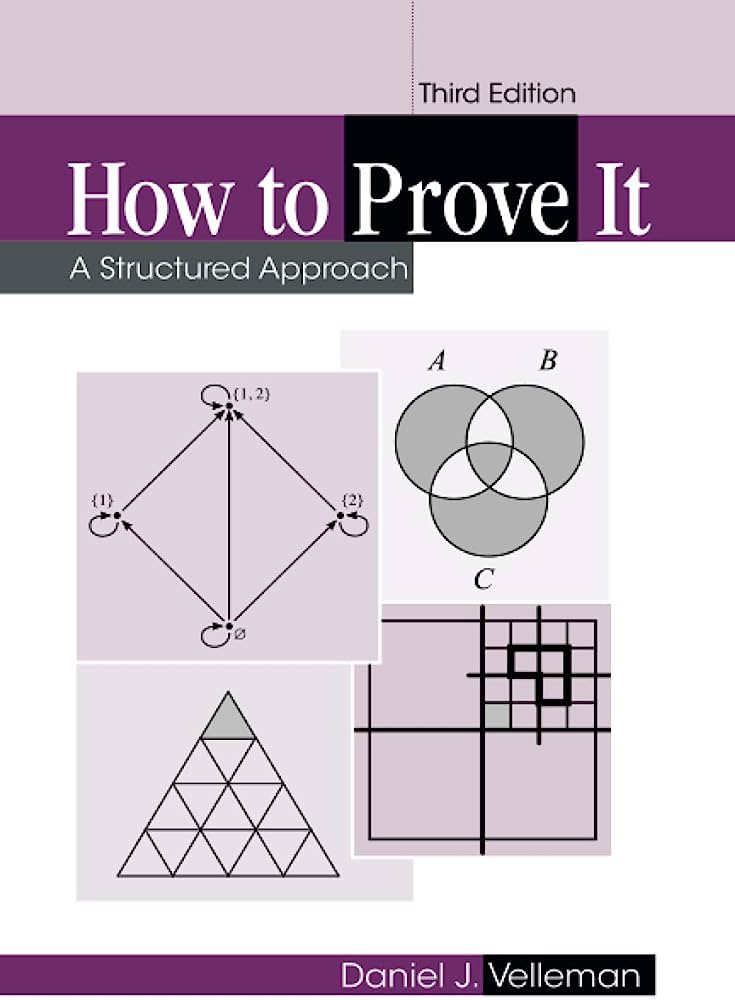
\includegraphics[width=0.4\textwidth]{htp.jpg}
    \\
    \vspace{1cm}
    \Huge{\bf Introduction}
\end{center}
\newpage
\begin{enumerate}
    % Exercise 1
    \item 
        (a) Factor $2^{15} - 1 = 32,767$ into a product of two smaller positive integers.\\\\
         a. The proof of conjecture 2 gives us a method for transforming 32, and 767 into a product of two smaller positive integers. The book gave us this important data:
         \begin{itemize}
              \item
              if $n$ is not prime $\Rightarrow 2^n - 1$ must also not be prime
              \item  
              Since $n$ is not prime, there are positive integers $a$ and $b$ such that $a<n$, $b<n$, and $n = a * b$. Let $x = 2^b - 1$ and $y = 1+ 2^b + 2^{2b} + ... + 2^{(a-1)b}$.
        \end{itemize}
         The proof is in the book but the conclusion is that \textbf{$x * y = 2^n - 1$}
         \\
         So if we want to know the two numbers that produce 32,767 we need to do the following:\\
         $n = 15$ and $15 = 3 * 5$, then we could say $a = 3$ and $b = 5$, so\\ $x = 2^5 - 1 = 31$ and\\ $y = 1 + 2^b + 2^{(a-1)b} = 1 + 2^b + 2^{2b} = 1 + 2^5 + 2^{10} = 1057\\ \Longrightarrow 32,767 = 31 * 1057$. 
         \\\\
        (b) Find an integer x such that $1 < x < 2^{32,767}- 1$ and $2^{32,767}- 1$ is divisible by x.\\\\
        b. $2^{32,767}- 1$ can be expressed like this $2^{31*1057}- 1$ that is equal to $x*y$ being $x =2^{31} - 1$, and $y = 1 + 2^{31} + 2^{2*31} + ... + 2^{1056*31}$. So the answer can either be $x$ or $y$.
        
    
    % Exercise 2 -- For some reason, my conjectures differ from those in the original solution manual.
    \item 
        Make some conjectures about the values of n for which $3^{n} - 1$ is prime or
        the values of n for which $3^{n}- 2^{n}$ is prime. (You might start by making a
        table similar to Figure 1.)
        \begin{center}
             \begin{tabular}{c | c | c | c | c | c} 
                 n & Primality of n & $3^{n} - 1$ & Primality of $3^{n} - 1$ & $3^{n}- 2^{n}$
                 & Primality of $3^{n} - 2^{n}$ \\ [1ex] 
                 \hline
                 2 & Prime & 8 & Composite & 5 & Prime\\ 
                 \hline
                 3 & Prime & 26 & Composite & 19 & Prime\\
                 \hline
                 4 & Composite & 80 & Composite & 65 & Composite\\
                 \hline
                 5 & Prime & 242 & Composite & 211 & Prime\\
                 \hline
                 6 & Composite & 728 & Composite & 665 & Composite\\
                 \hline
                 7 & Prime & 2186 & Composite & 2059 & Prime\\
                 \hline
                 8 & Composite & 6560 & Composite & 6305 & Composite\\
                 \hline
                 9 & Composite & 19682 & Composite & 19171 & Prime\\
                 \hline
                 10 & Composite & 59048 & Composite & 58025 & Composite\\
                 \hline
            \end{tabular}
        \end{center}
        \textbf{Conjecture 1:} Suppose n is an integer larger than one and n is prime. Then $3^{n}- 1$ is not prime, and $3^{n}- 2^{n}$ is prime. \\\\
        \textbf{Conjecture 2:} Suppose n is an integer larger than one and n is not prime. Then $3^{n}- 1$ is not prime.

    % Exercise 3
    \item 
        The proof of Theorem 3 gives a method for finding a prime different
        from any in a given list of prime numbers.\\\\
        (a) Use this method to find a prime different from 2, 3, 5, and 7.\\\\
        Euclid's theorem presents a method based on the fact: "Every integer larger than 1 is either prime or can be written as a product of two or more primes". The logic is that, with a list of prime numbers, if we add one to the result of their multiplication it can happen two things. The first one is that the result is a prime number (cannot be divided by any smaller prime number).
        And the second one is that we do not obtain a prime number (the number be divided) then we can construct the result with two prime numbers \textbf{different from the ones on the list} cause the result cannot be divided by any of the prime numbers given in the list 'cause of the 1 that is being added. In either case, we finally discover at least one prime number that is not on the list.
        
        a. In this case $2 * 3 * 5 * 7 + 1 = \textbf{211}$ that is indeed prime.
        \\\\
        (b) Use this method to find a prime different from 2, 5, and 11.
        \\\\
        b. $2 * 5 * 11 + 1= 111$. We realize 111 can be divided by 3, so it is not a prime number. In this process, we found that $111 = \textbf{3 * 37}$ both prime numbers.
    
    % Exercise 4
    \item
        Find five consecutive integers that are not prime.\\\\
        Before understanding that this exercise was referring to a formula given in the book,
        I thought of a simple example, the five numbers: 24, 25, 26, 27, and 28. Now
        the point of the exercise was to use the method given in theorem 4.
        \textit{"For every positive integer n, there is a sequence of n consecutive positive integers
        containing no primes"}. The sequence is represented this way: $first\_sequence\_number = (n + 1)! + 2$. So if we wanna find out \textbf{five} numbers in a row that are not prime, we need to do the math with n = 5 until $first\_sequence\_number + (n - 1)$.\\
        $first\_sequence\_number = 6! + 2 = 722$. So the five numbers are \textbf{722, 723, 724, 725, 726}.
    
    % Exercise 5
    \item
        Use the table in Figure 1 and the discussion on p. 5 to find two more perfect
        numbers.\\\\
        Mersenne primes have the following form: $2^{n}-1$. Euclid's Theorem states that if we have a Mersenne prime, and then we multiply it by $2^{n-1}$ we obtain a perfect number:\\
        We know from the table on page 5 that with n = 5, and n = 7 we can form two Mersenne primes. So:\\
        For n = 5 we have $(2^{5-1})(2^{5}-1) = 16*31 =$ \textbf{496} (Perfect Number)\\
        For n = 7 we have $(2^{7-1})(2^{7}-1) = 64*127 =$ \textbf{8128} (Perfect Number)
    
    % Exercise 6
    \item
        The sequence 3, 5, and 7 is a list of three prime numbers such that each pair of
        adjacent numbers in the list differ by two. Are there any more such “triplet
        primes”?\\\\
        There are no more "triplet primes" because the remainder when any integer $n > 3$ is divided by 3 will be either 0, 1, or 2. If it is 0, then n is divisible by 3, so it is composite. If it is 1, then n + 2 is divisible by 3 and therefore composite. If it is 2, then n + 4 is divisible by 3 and composite. Thus, the numbers n, n + 2, and n + 4 cannot all be prime. (Answer from the solution's manual)

    % Exercise 7
    \item
        A pair of distinct positive integers (m, n) is called amicable if the sum of all positive integers smaller than n that divide n is m, and the sum of all positive integers smaller than m that divide m is n. Show that (220, 284) is amicable.\\\\
        The positive integers smaller than 220 that divide 220 are 1, 2, 4, 5, 10, 11, 20, 22, 44, 55, and 110, and 1 + 2 + 4 + 5 + 10 + 11 + 20 + 22 + 44 + 55 + 110 = 284. The positive integers smaller than 284 that divide 284 are 1, 2, 4, 71, and 142, and 1 + 2 + 4 + 71 + 142 = 220.
\end{enumerate}
\end{document}

